% Configuración del tipo páginas
	\documentclass[11pt, a4paper,english,spanish]{article}
	\parindent = 11pt
	\parskip = 0 pt	
	\usepackage[width=15.5cm, left=3cm, top=2.5cm, height= 24.5cm]{geometry}

% Paquete para reconocer la separación en sílabas en español
	\usepackage[utf8]{inputenc}
	\usepackage[spanish]{babel}

% Paquetes especiales
	\usepackage{amsmath}
	\usepackage{amsthm} %paquete para teoremas y propiedades
	\usepackage{amsfonts}
	\usepackage{amssymb}
	\usepackage[pdftex]{graphicx}
	\usepackage{float}
	\usepackage{graphicx} %paquete para incluir imagenes

	\usepackage{caption}
	\usepackage{subcaption}


\usepackage{algorithm}
\usepackage{algorithmicx}
\usepackage{algpseudocode}
\usepackage{tabularx}
\usepackage{multirow}

% Paquete para incluir hypervinculos
	\usepackage{color}
	\usepackage{url}
	\definecolor{lnk}{rgb}{0,0,0.4}
	%colores para la inclusion del codigo
	\definecolor{gray97}{gray}{.97}
	\definecolor{gray75}{gray}{.75}
	\definecolor{gray45}{gray}{.45}
	\usepackage[colorlinks=true,linkcolor=lnk,citecolor=black,urlcolor=black]{hyperref}

	\newcommand{\todo}{\textbf{\textcolor{red}{TODO: }}}

% Paquete para armar índices
	\usepackage{makeidx}
	\makeindex

\renewcommand{\thefootnote}{\arabic{footnote}} %config de footnote

%Paquete y su config para incluir los codigos de c++
\usepackage{times}
\usepackage{listings}


\lstset{ frame=Ltb,
framerule=0pt,
aboveskip=0.5cm,
framextopmargin=3pt,
framexbottommargin=3pt,
framexleftmargin=0.4cm,
framesep=0pt,
rulesep=.4pt,
backgroundcolor=\color{gray97},
rulesepcolor=\color{black},
tabsize=2,
%
stringstyle=\ttfamily,
showstringspaces = false,
basicstyle=\scriptsize\ttfamily,
commentstyle=\color{gray45},
keywordstyle=\bfseries,
language=C++,
%
numbers=left,
numbersep=15pt,
numberstyle=\tiny,
numberfirstline = false,
breaklines=true,
}

\lstset{emph={%  
    Coord, SolucionEj1, SolucionEj2%
    }, emphstyle={\bfseries}%
}%

% minimizar fragmentado de listados
\lstnewenvironment{listing}[1][]
{\lstset{#1}\pagebreak[0]}{\pagebreak[0]}

\lstdefinestyle{C++}
{language=C++}

\lstdefinestyle{Python}
{language=Python}

	
% Carátula
	\usepackage{caratula}

	%\usepackage[vlined,tworuled,commentsnumbered,linesnumbered]{algorithm2e}

% Más espacio entre líneas
	\parskip=1.5pt

\newcommand{\comment}[1]{\emph{// {#1}\;}} 
\newcommand{\la}{\(\leftarrow\)}
\newcommand{\ra}{\(\rightarrow\)}

\hypersetup{ 
pdfauthor = {},
pdftitle = {}, 
pdfkeywords = {},
pdfstartview={XYZ null null 0.80},
}

\begin{document}
\titulo{TP1: Wiretapping}
%\subtitulo{Grupo ???}
%\resumen{
%	\textbf{Resumen: } \\ \\
%	\indent \textbf{Keywords: }
%}
\fecha{Fecha de entrega: 29 de Abril}
\materia{Teoría de las Comunicaciones}
\integrante{Ignacio Gleria}{387/10}{igleria@dc.uba.ar}
\integrante{Patricio Mosse}{515/06}{patricio.mosse@gmail.com}
\integrante{David Temnyk}{779/10}{dtemnyk@dc.uba.ar}
\integrante{Gustavo Torrecilla}{833/10}{gustavo.d.t\_90@hotmail.com}

\maketitle
% Índice
\newpage \printindex \tableofcontents
\normalsize

\newpage

\section{Introducción}

En este trabajo práctico hemos desarrollado una herramienta de diagnóstico de red con el objetivo de capturar los paquetes que se envían a través de la misma, identificar los distintos protocolos utilizados y principalmente, analizar el tráfico ARP (\textit{Address Resolution Protocol}) mediante herramientas provistas por la teoría de la información. Este protocolo permite vincular identificadores de la capa de enlace (MAC) con direcciones de la capa de red (IP) de dispositivos conectados a una red local.


Hemos utilizado el lenguaje de programación Python para el desarrollo de la herramienta, valiéndonos principalmente del software de manipulación de paquetes Scapy. La captura de paquetes fue realizada sobre 4 redes que... \textbf{TODO:} Definir cuáles van a ser...


\newpage
\subsection{Modelos de fuente de información}
\label{subsec:modelos-fuente-informacion}

Para analizar las redes locales estudiadas, utilizamos dos modelos de fuente de información:
\vspace*{-2mm}

\begin{itemize}
  \item $S_{dst}$ = \{$s_1$ $\cdots$ $s_n$\}, siendo $s_i$ una IP que aparece como dirección destino en los paquetes ARP \emph{who-has}.
  \item $S_{src}$ = \{$s_1$ $\cdots$ $s_n$\}, siendo $s_i$ una IP que aparece como dirección origen en los paquetes ARP \emph{who-has}.
\end{itemize}

Esto permitió, dado el flujo de paquetes de una red local, definir la \textbf{información} del evento $E_i$: ``aparición del símbolo $s_i$'' como:

$$I (E_i) = log\left(\frac{1}{P(E_i)}\right)$$

unidades de información, donde $P(E_i)$ es la probabilidad de que suceda $E_i$. Al usar $log_2$, la unidad obtenida se denomina bits.

Utilizando la definición previa se puede definir la \textbf{entropía} de una fuente ($S_{dst}$ o $S_{src}$ por ejemplo), representada por $H(S)$, como el valor medio ponderado de la cantidad de información de la aparición de cada símbolo $s_i$ que la compone.

$$H(S) = \sum_{i=1}^{n} P(E_i)\,I(E_i) = \sum_{i=1}^{n} P(E_i)\,log\left(\frac{1}{P(E_i)}\right)$$

Adicionalmente, en base a estas nociones podemos establecer un criterio para considerar que un nodo de la red se considera un \textbf{nodo distinguido} para una fuente dada: un nodo es distinguido cuando la información asociada a la aparición de su IP es menor que la entropía de dicha fuente.

\subsection{Grafo de relación entre los nodos}
\label{subsec:grafo-relacion-nodos}

Como los paquetes ARP tienen una dirección IP fuente y una dirección IP destino, surge naturalmente la siguiente relación entre IP's: IP $x$ a IP $y$ \emph{sii} se observó algún paquete ARP con dirección fuente IP $x$ y dirección destino IP $y$.

Por lo tanto, en base a una muestra de paquetes ARP de una LAN, podemos definir el grafo de relación entre los nodos en base a la relación anterior, proveyendo una noción complementaria de \textbf{nodo distinguido}, para aquellos nodos que tengan grados de entrada y/o salida muy elevados.
\newpage
\section{Experimentación}
La experimentación consistió en capturar el tráfico de paquetes, utilizando la herramienta previamente desarrollada, en las siguientes redes: una red hogareña, un McDonalds, un Starbucks, el laboratorio del DC y en el Subte.

La herramienta desarrollada no solo captura el tráfico de paquetes, sino que también hace una distinción de tipos de paquetes (qué protocolos usan), y en caso de que sean ARP toma su IP destino. Luego, con esta información se procede a calcular las probabilidades de aparición de cada tipo de paquete, contando la cantidad de apariciones de un paquete sobre el total de los paquetes capturados. De manera análoga se calcula las probabilidades de aparición de las IPs destino en los paquetes ARP. Una vez calculadas las probabilidades, es fácil realizar el cálculo de información de cada evento y las entropías de las distintas fuentes, aplicando las fórmulas presentadas en la sección de \textit{Desarrollo}.

Luego se realizaron histogramas para tener una visualización de la cantidad de apariciones de cada evento, asi también como la información de los mismos.
Por último, realizamos un grafo que representa el tráfico de paquetes en cada red, para poder comprender con mayor claridad lo que sucede en ellas.

\newpage

\subsection{Red Hogareña}

En este experimento, capturamos los paquetes de la LAN de uno de los miembros de nuestro grupo. La medición fue realizada un día sábado desde las 12 hs hasta las 14 hs. La cantidad de paquetes capturados aproximadamente es de 125000. Sin embargo, sólo 153 de estos corresponden al protocolo ARP.

\newpage

\subsection{Red McDonald's}

Para el siguiente experimento, capturamos los paquetes de la LAN Wi-Fi pública del McDonald's ubicado en el shopping Alto Avellaneda. La medición fue realizada un día sábado desde las 18 hs hasta las 20 hs. La cantidad de paquetes capturados es de aproximadamente 65.000. De todos estos, sólo 918 corresponden al protocolo ARP.

\begin{figure}[H]
       \centering
       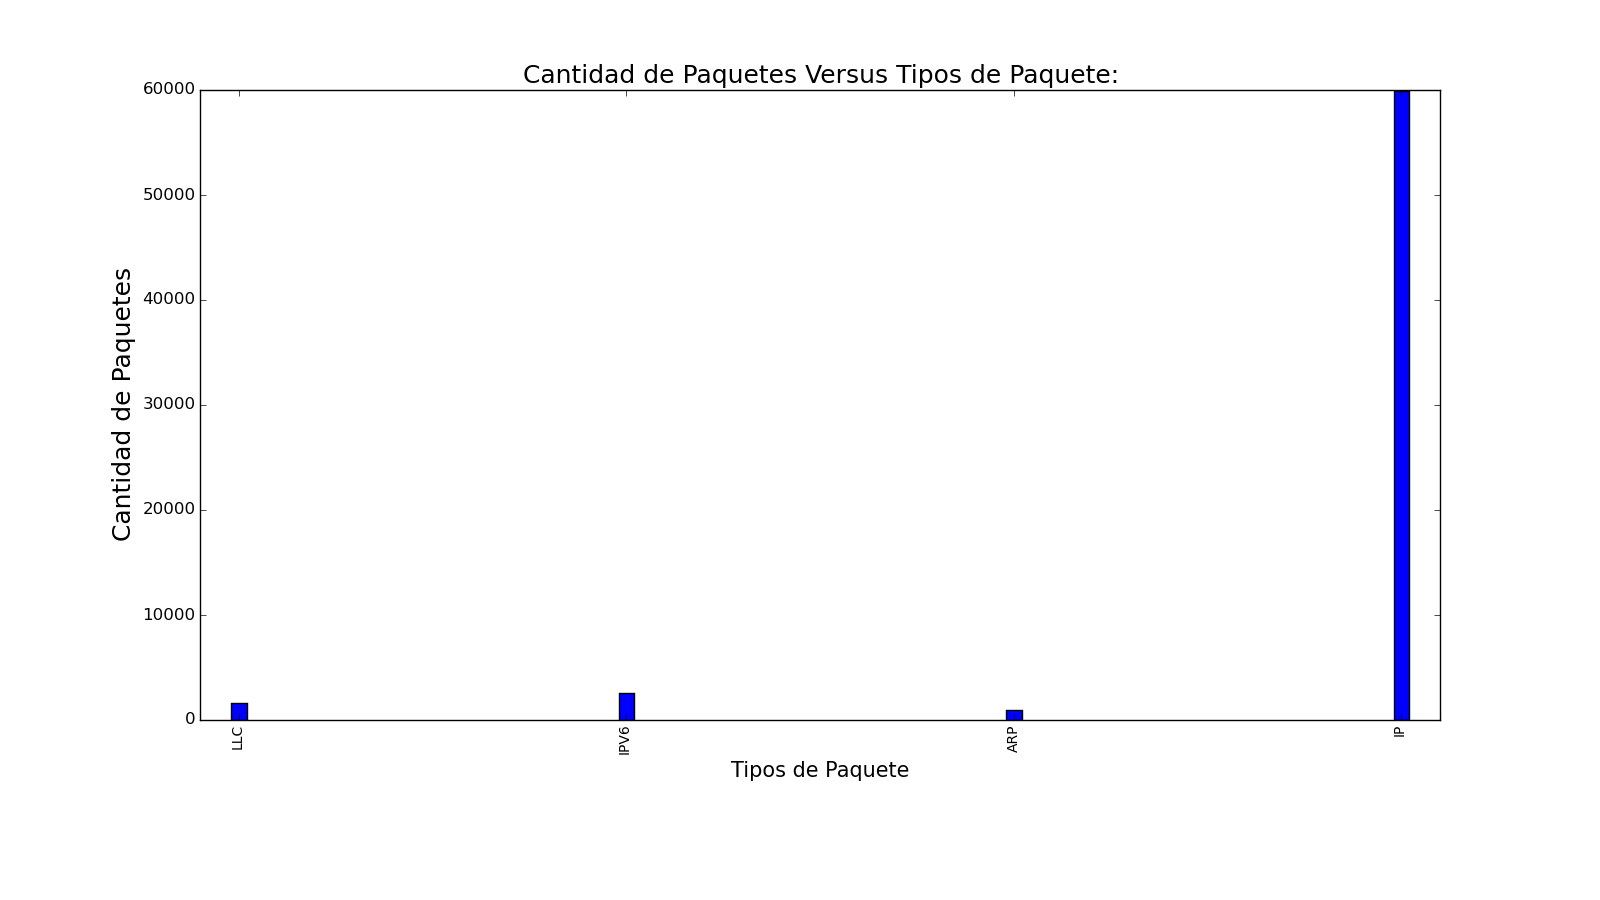
\includegraphics[width=1\textwidth]{../resultados/McDonalds/histogram_types.png}
       \caption{Protocolos de los paquetes capturados}
       \label{red-hogarena-types}
\end{figure}

\begin{figure}[H]
       \centering
       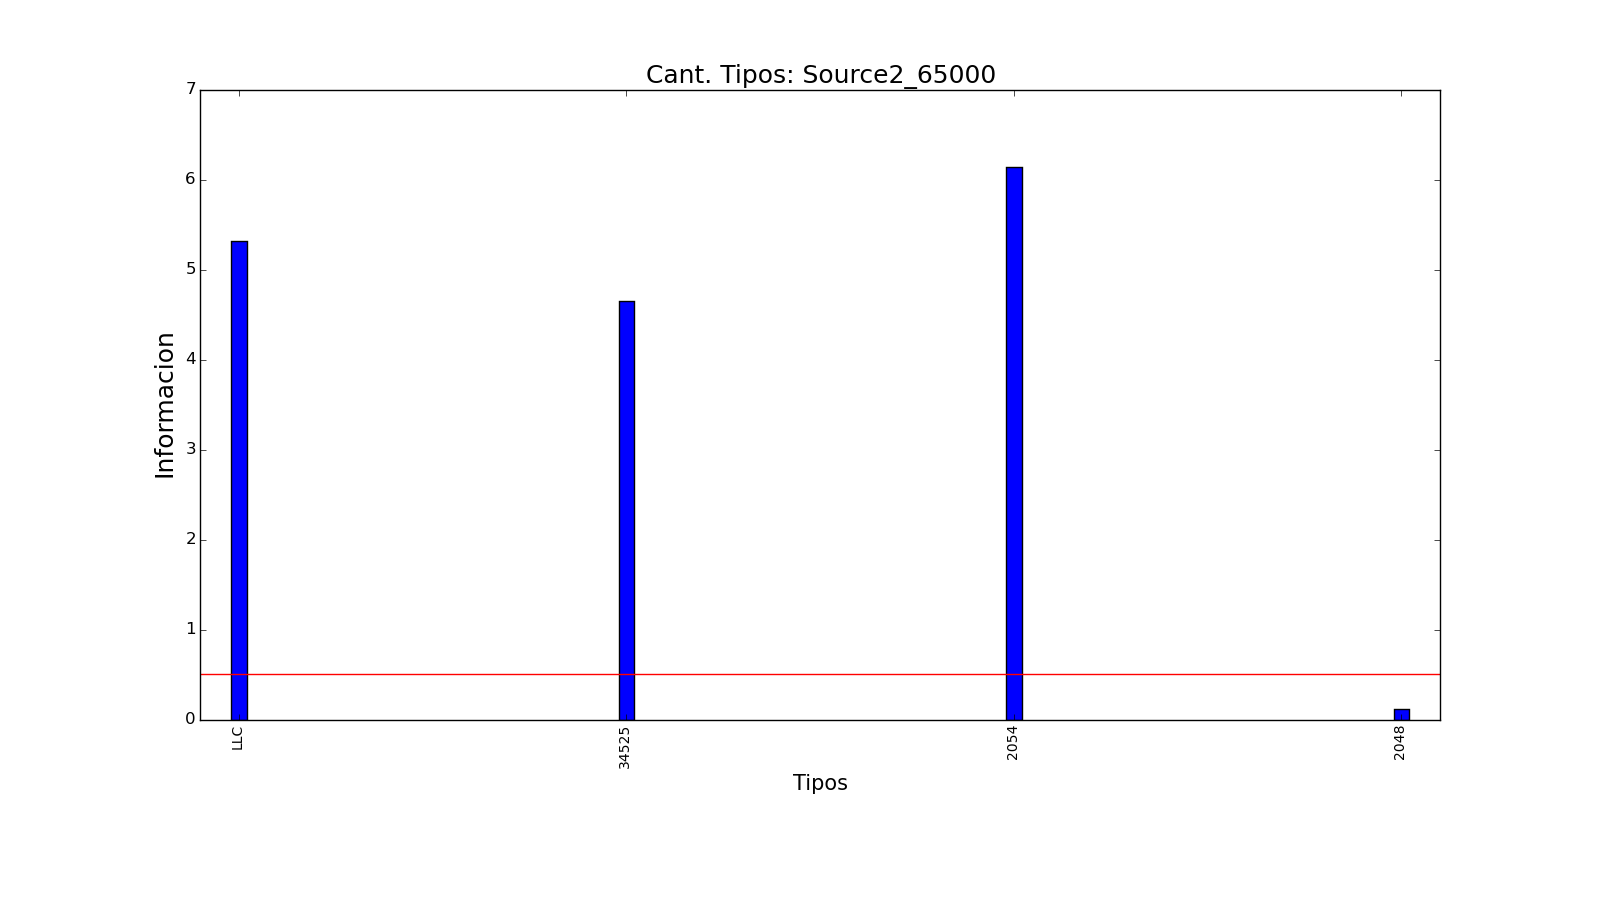
\includegraphics[width=1\textwidth]{../resultados/McDonalds/histogram_types_information.png}
       \caption{Información de los protocolos de los paquetes capturados}
       \label{red-hogarena-types}
\end{figure}


\newpage

\subsection{Red Starbucks}



\newpage

\subsection{Red Laboratorios DC}

Para este experimento, capturamos los paquetes de la LAN Wi-Fi Laboratorios-DC del Departamento de Computació de la FCEyN de la UBA. La medición fue realizada un día Lunes desde las 15hs y durante 15 minutos. La cantidad de paquetes capturados es de 4000. De estos, 164 corresponden al protocolo ARP.

\begin{figure}[H]
       \centering
       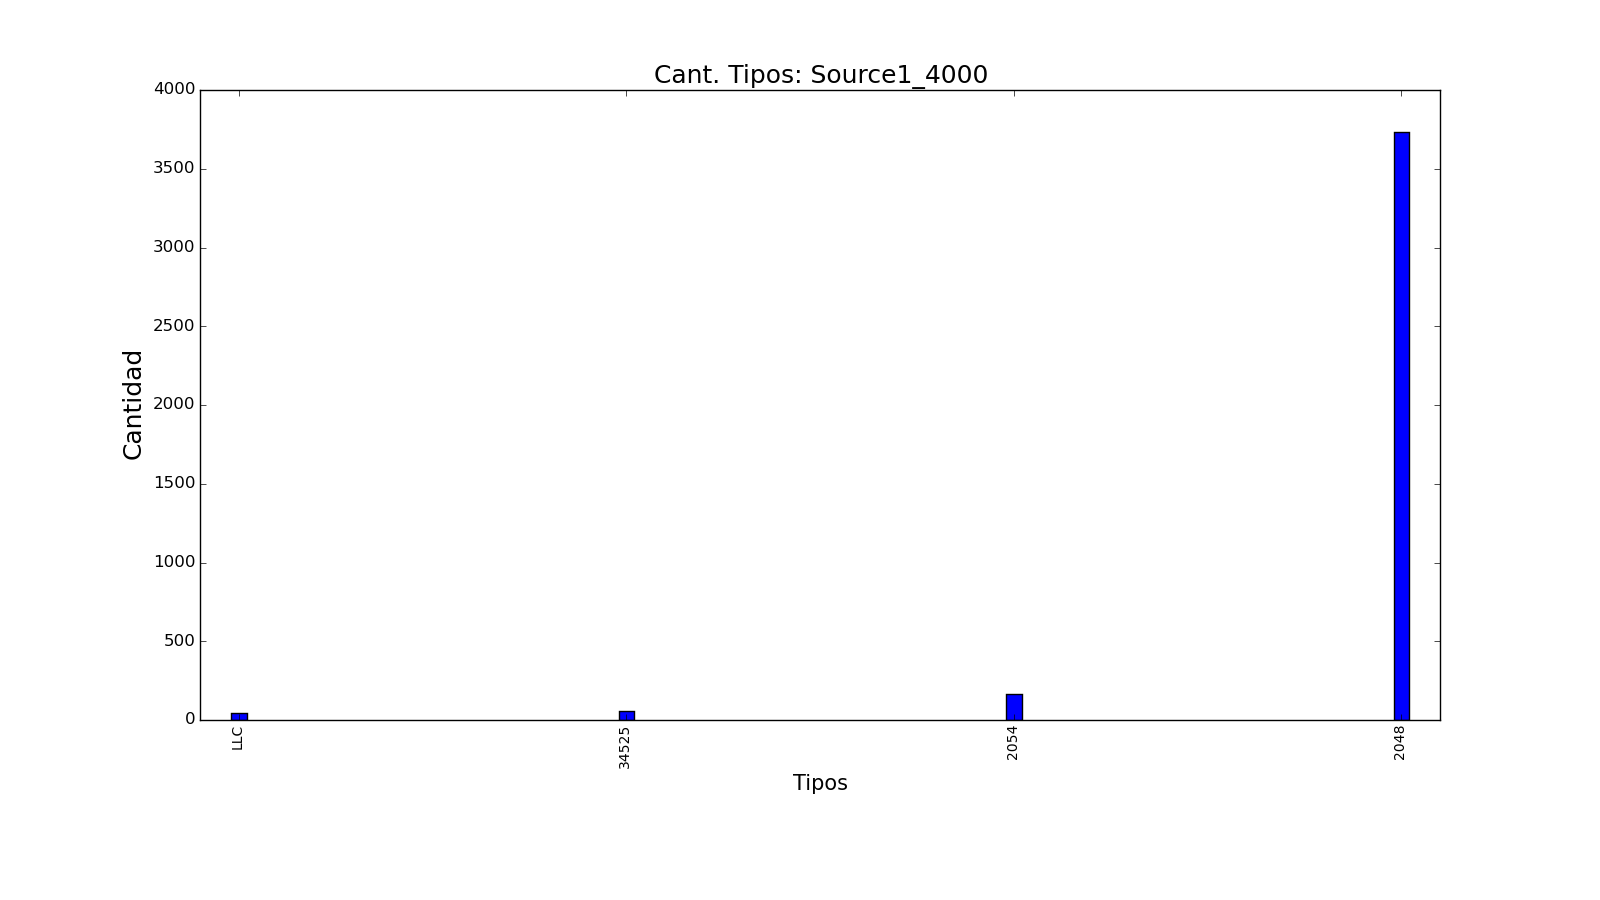
\includegraphics[width=1\textwidth]{../resultados/labo-corrida3/histogram_types.png}
       \caption{Protocolos de los paquetes capturados}
       \label{red-Starbucks-types}
\end{figure}

\begin{figure}[H]
       \centering
       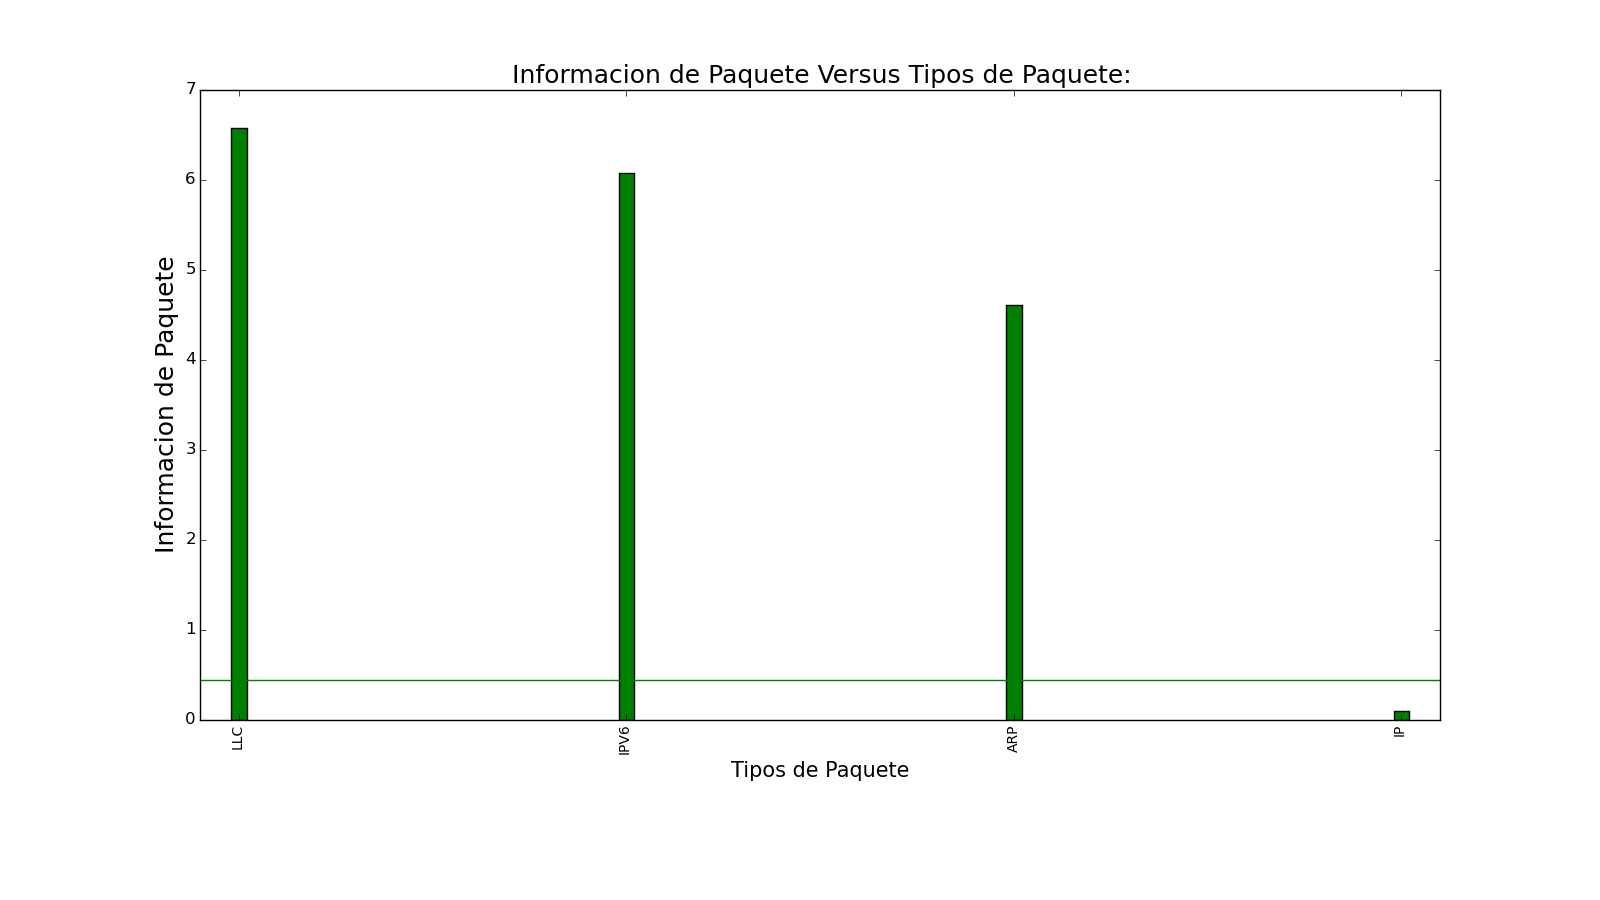
\includegraphics[width=1\textwidth]{../resultados/labo-corrida3/histogram_types_information.png}
       \caption{Información de los protocolos de los paquetes capturados}
       \label{red-Starbucks-types-information}
\end{figure}

Como podemos observar también en este experimento, de acuerdo a nuestra definición de protocolo distinguido, el protocolo IPv4 sería el único distinguido en esta fuente. Es razonable, ya que la cantidad de paquetes IPv4 es mucho mayor que la cantidad de paquetes IPv6, LLC y ARP. La información de los paquetes IPv4 es \textbf{0.0988917569855}, mientras que la entropía de la fuente es \textbf{0.440025436837}. Se observa como la información es claramente menor a la entropía.

\begin{figure}[H]
       \centering
       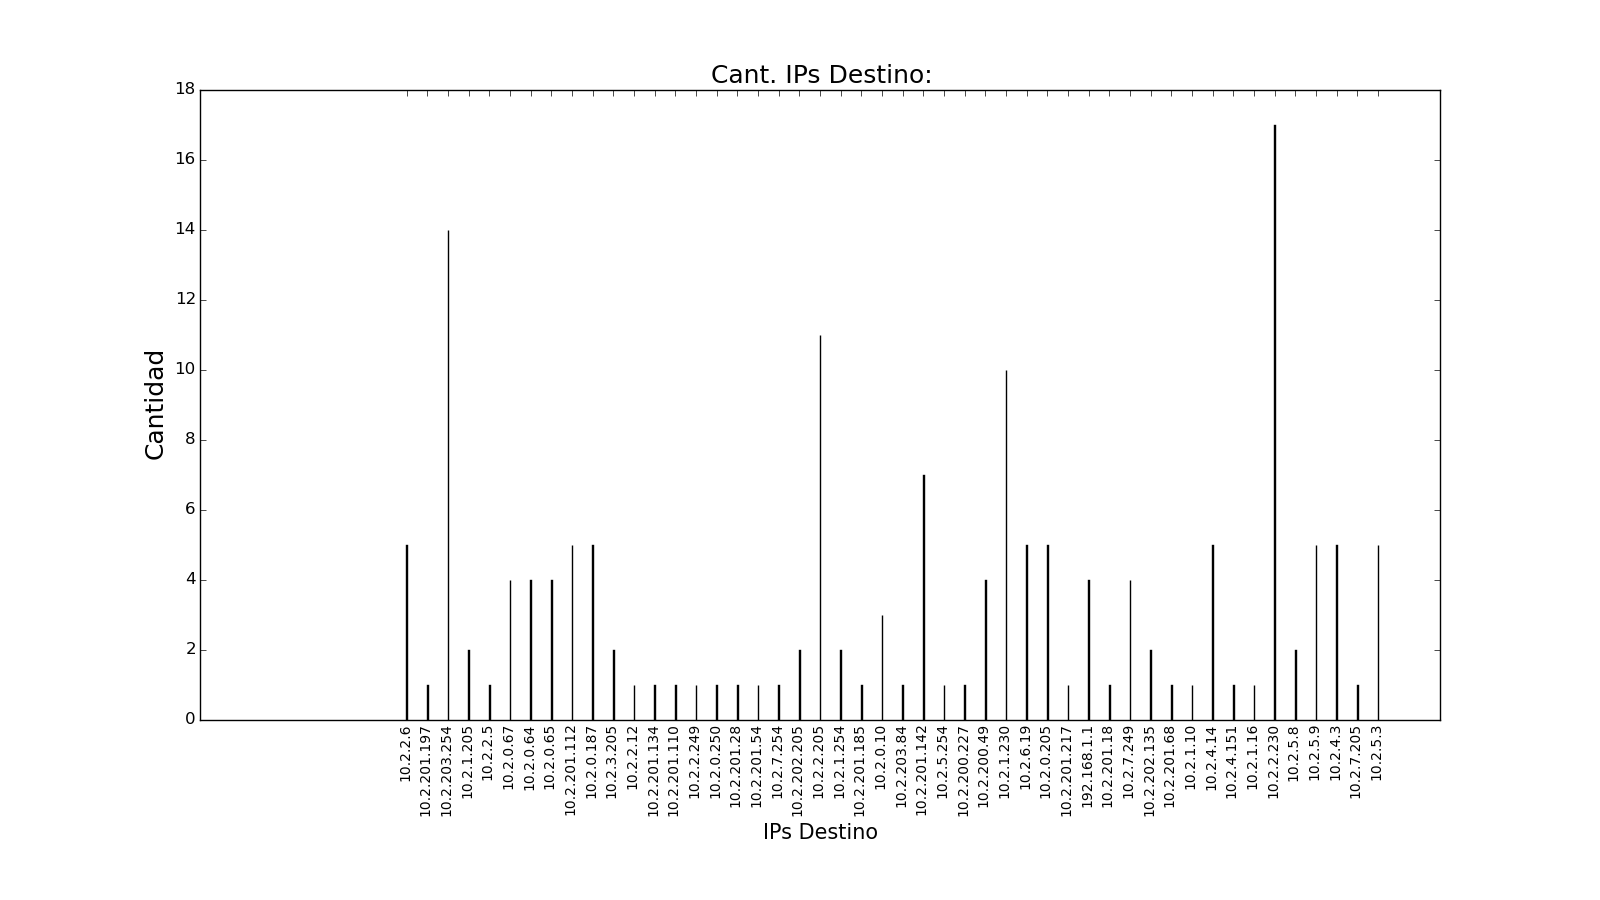
\includegraphics[width=1\textwidth]{../resultados/labo-corrida3/histogram_dst.png}
       \caption{IPs destino de los paquetes ARP}
       \label{red-Starbucks-dst}
\end{figure}

\begin{figure}[H]
       \centering
       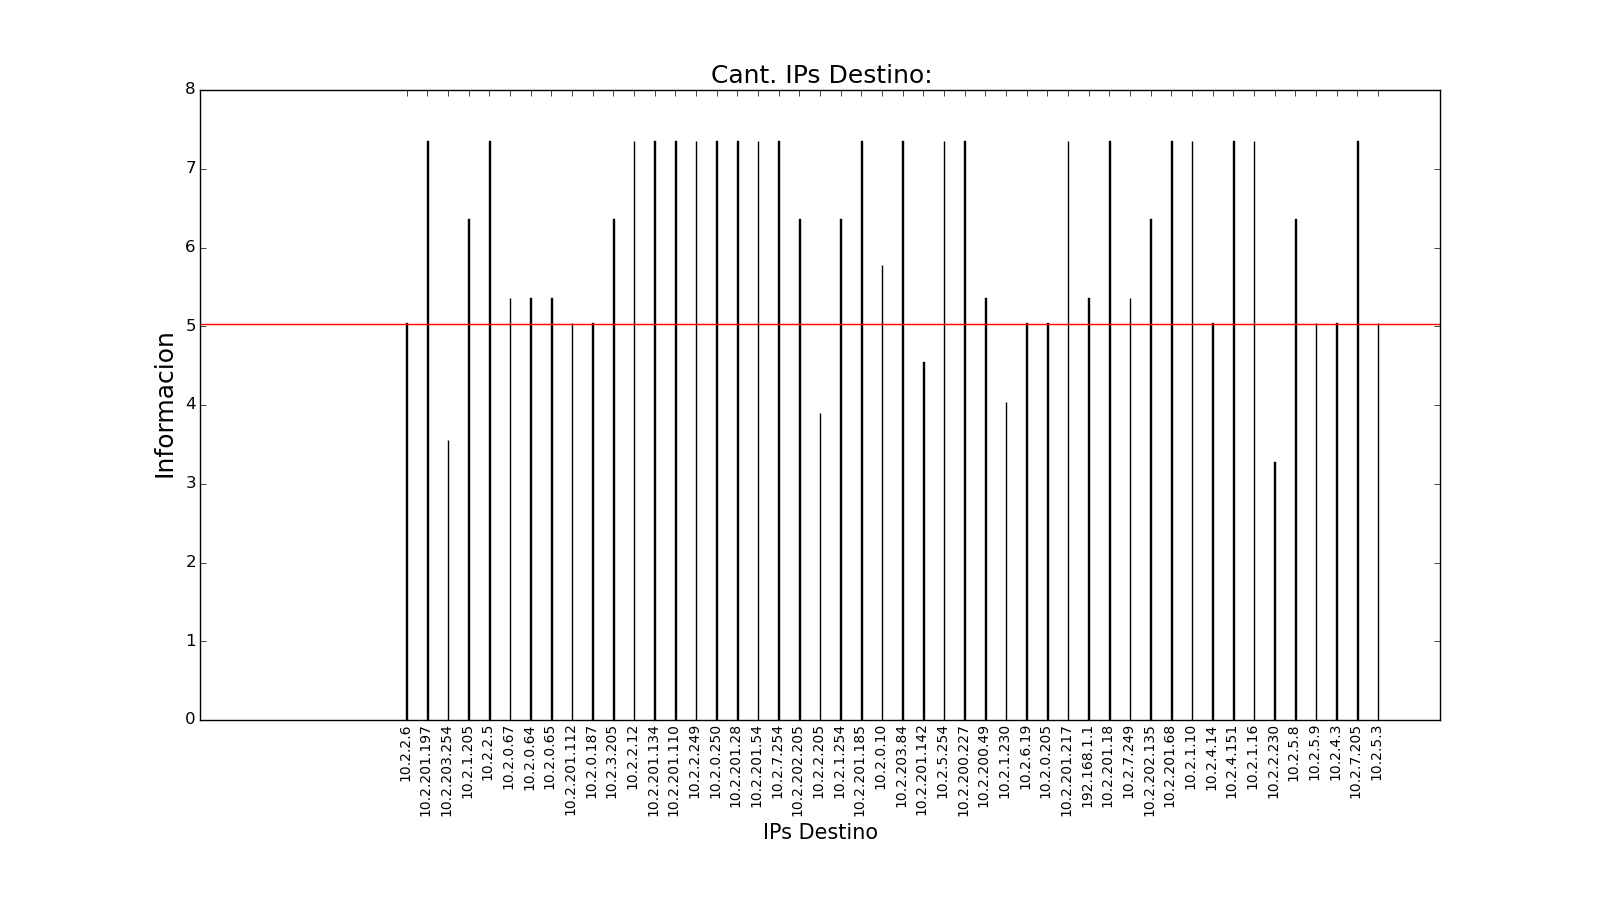
\includegraphics[width=1\textwidth]{../resultados/labo-corrida3/histogram_dst_information.png}
       \caption{Información de IPs destino de los paquetes ARP}
       \label{red-Starbucks-dst-information}
\end{figure}


\begin{figure}[H]
       \centering
       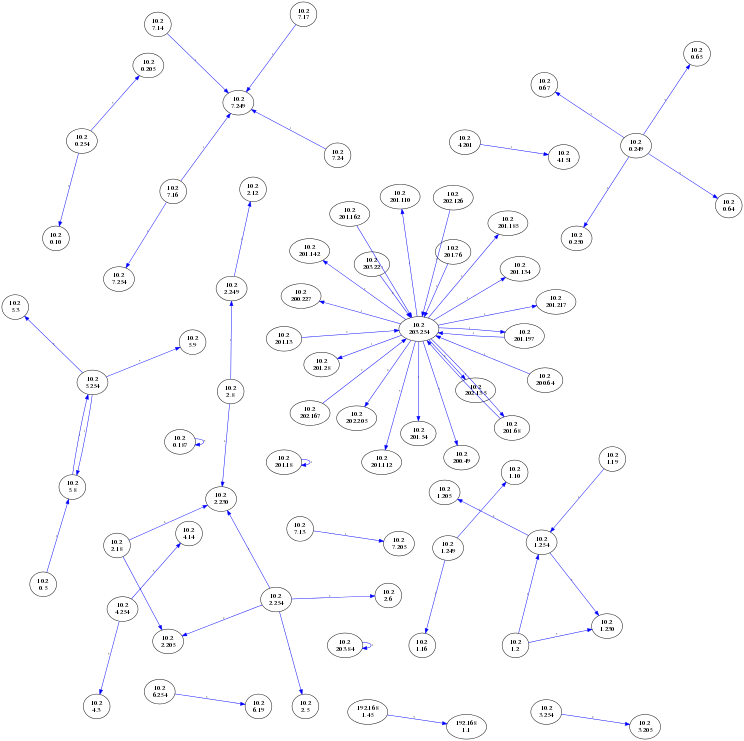
\includegraphics[width=1\textwidth]{../resultados/labo-corrida3/network.png}
       \caption{Tráfico de paquetes ARP}
       \label{red-Starbucks-dst-information}
\end{figure}

Analizando la información de estos gráficos vemos como la IP \textbf{10.2.203.254} parece ser el router: recibe una mayor cantidad de paquetes que casi todas las demás IPs, es un nodo distinguido por ser su información menor a la entropía, y las conexiones que tiene son a las IPs 10.2.200.X, 10.2.201.X y 10.2.202.X, que deben ser subnets.\\

También vemos por ejemplo que la IP \textbf{10.2.2.230} recibe incluso una mayor cantidad de paquetes y  también es un nodo distinguido, pero esa mayor cantidad de paquetes viene desde pocos nodos. Creemos por esto que puede tratarse de algún servidor (de datos, de imágenes, etcétera).

\newpage

\subsection{Red Subte D}

Para el último experimento, capturamos los paquetes de la LAN Wi-Fi Subte-BA de la estación Plaza Italia de la Línea D del Subte de Buenos Aires.La medición fue realizada un día Domingo a las 16.30hs y durante solamente 1 minuto (por motivos externos). Capturamos 1.000 paquetes de los cuales 25 son ARP.

\begin{figure}[H]
       \centering
       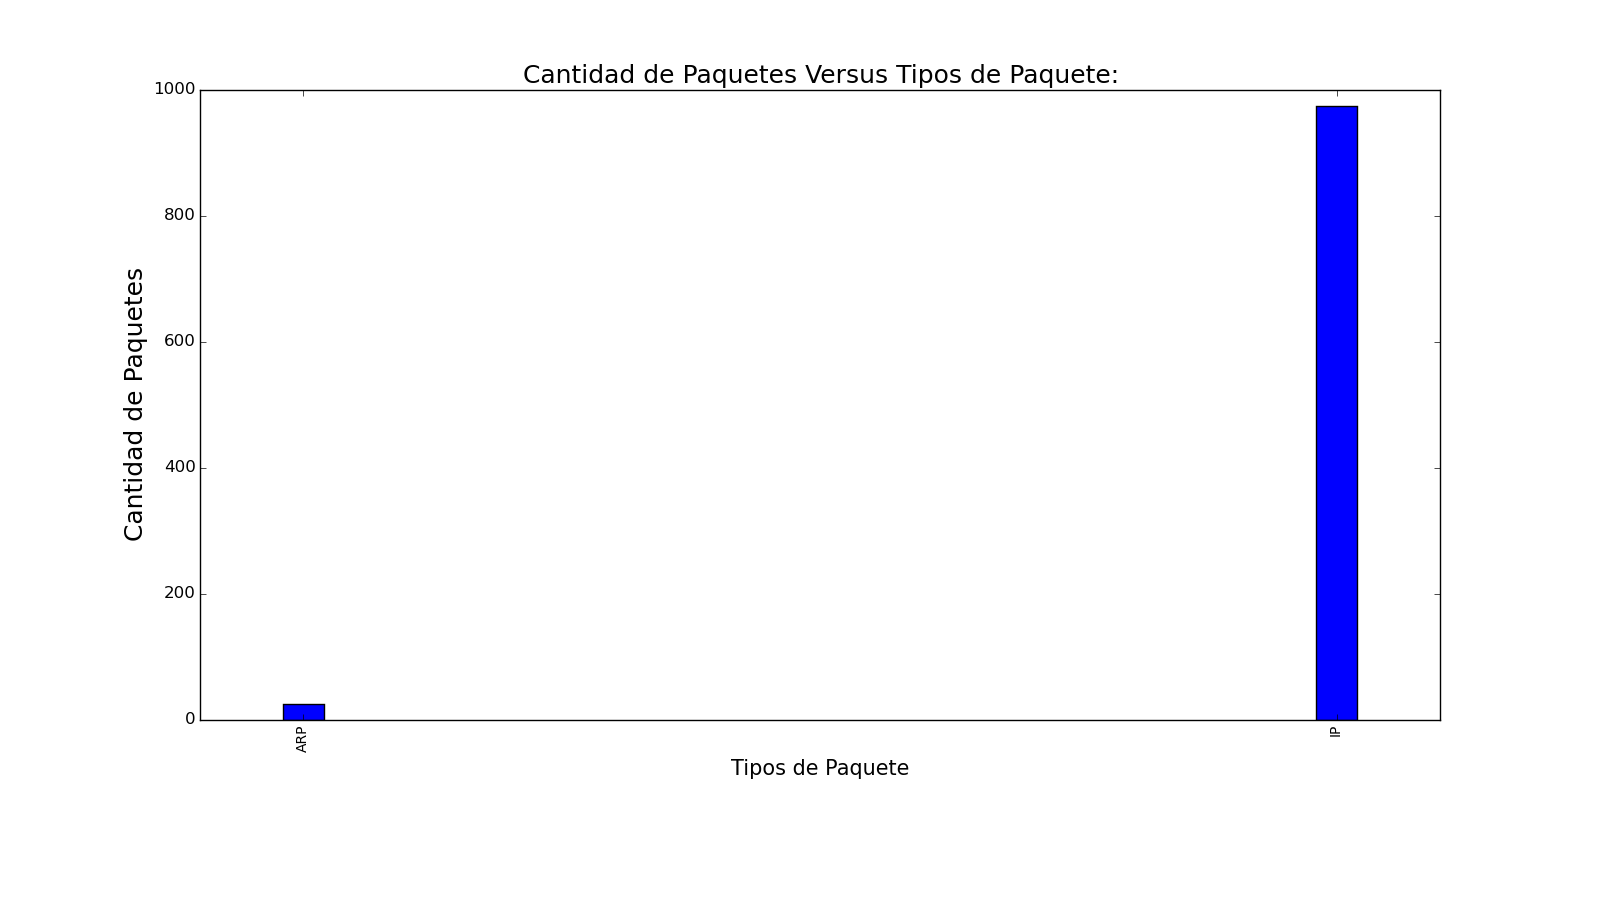
\includegraphics[width=1\textwidth]{../resultados/subte/histogram_types.png}
       \caption{Protocolos de los paquetes capturados}
       \label{red-Starbucks-types}
\end{figure}

En este caso el overhead impuesto por los paquetes ARP es de 2.5\%

\begin{figure}[H]
       \centering
       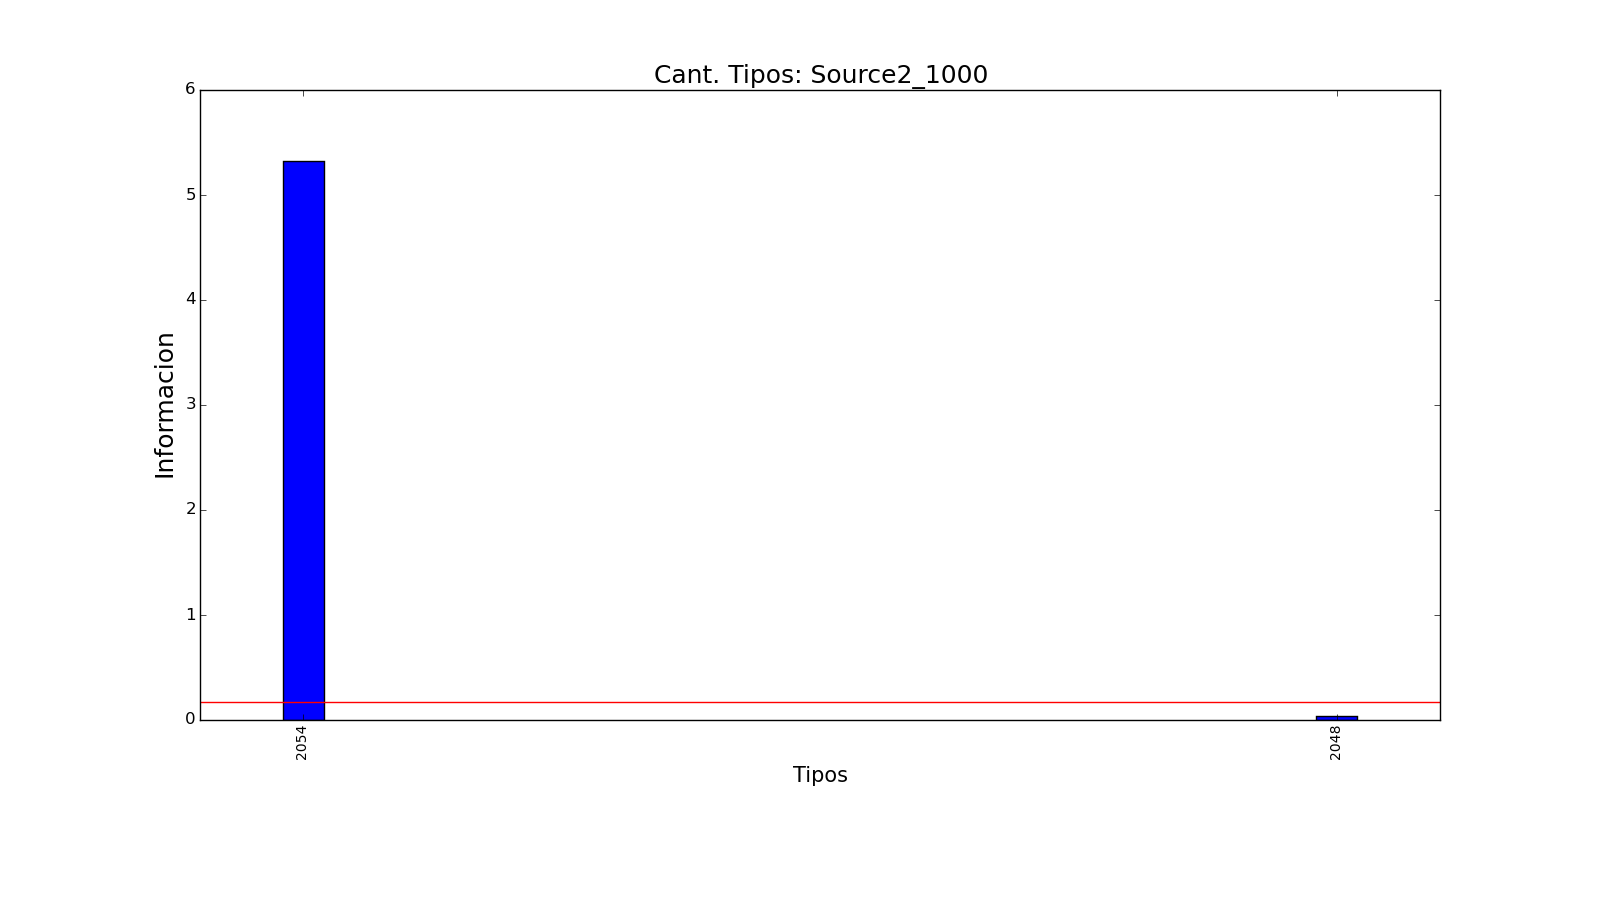
\includegraphics[width=1\textwidth]{../resultados/subte/histogram_types_information.png}
       \caption{Información de los protocolos de los paquetes capturados}
       \label{red-Starbucks-types-information}
\end{figure}

Como podemos también en este experimento, el protocolo IPv4 sería el único distinguido en esta fuente. Es razonable, ya que la cantidad de paquetes IPv4 es mucho mayor que la cantidad de paquetes ARP. La información de los paquetes IPv4 es \textbf{5.32192809489}, mientras que la entropía de la fuente es \textbf{0.168660931497}. Se observa como la información es muy menor a la entropía.

\begin{figure}[H]
       \centering
       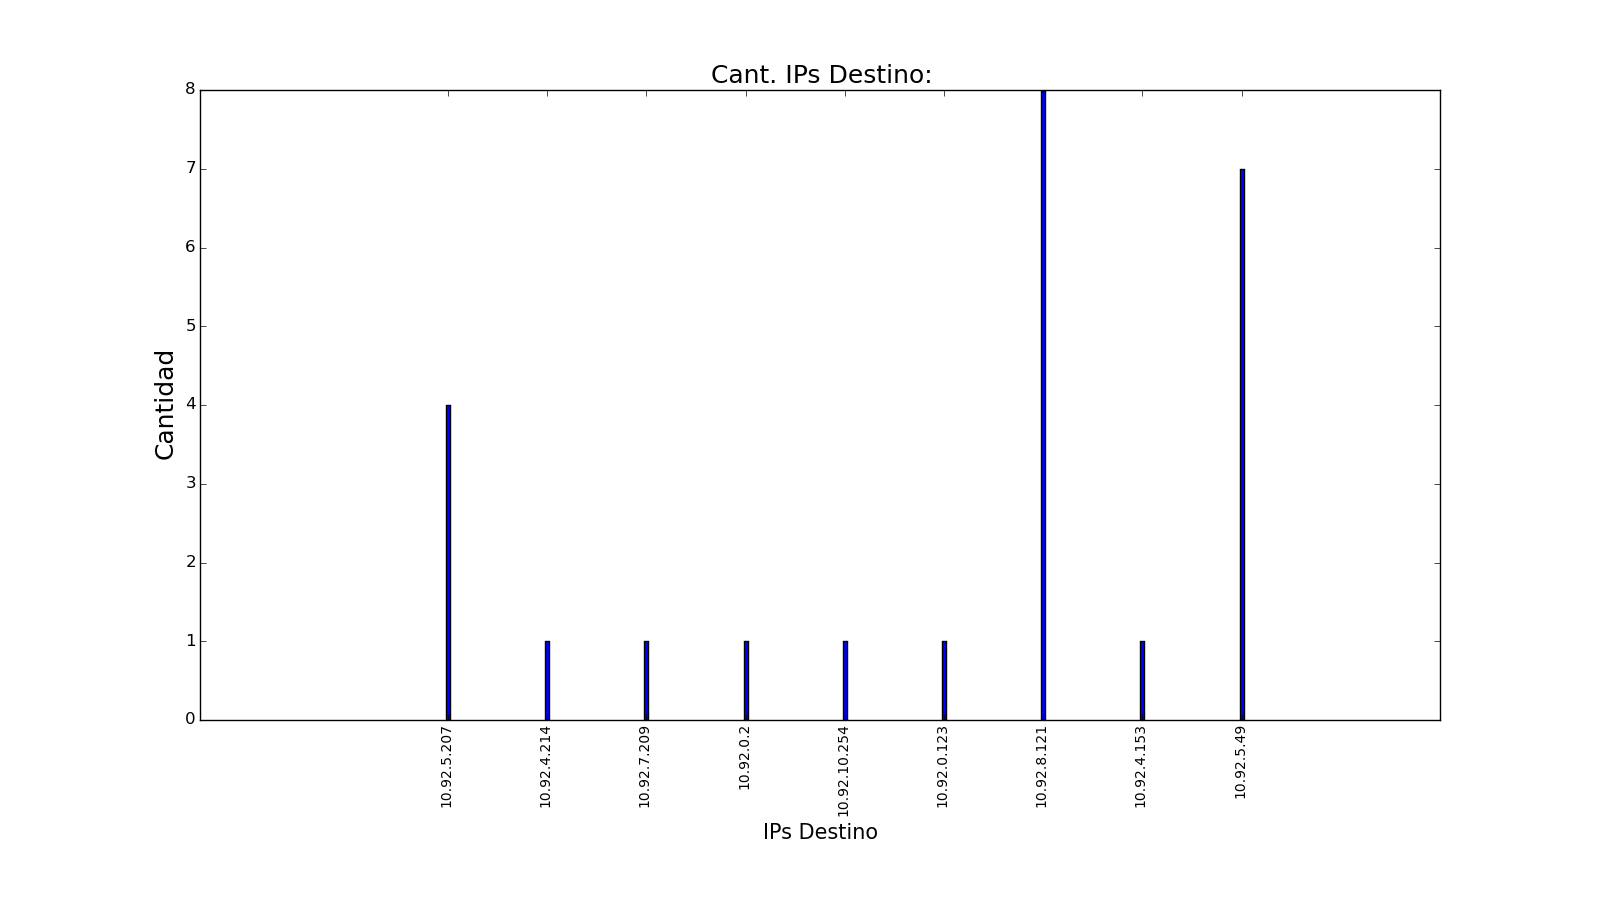
\includegraphics[width=1\textwidth]{../resultados/subte/histogram_dst.png}
       \caption{IPs destino de los paquetes ARP}
       \label{red-Starbucks-dst}
\end{figure}

\begin{figure}[H]
       \centering
       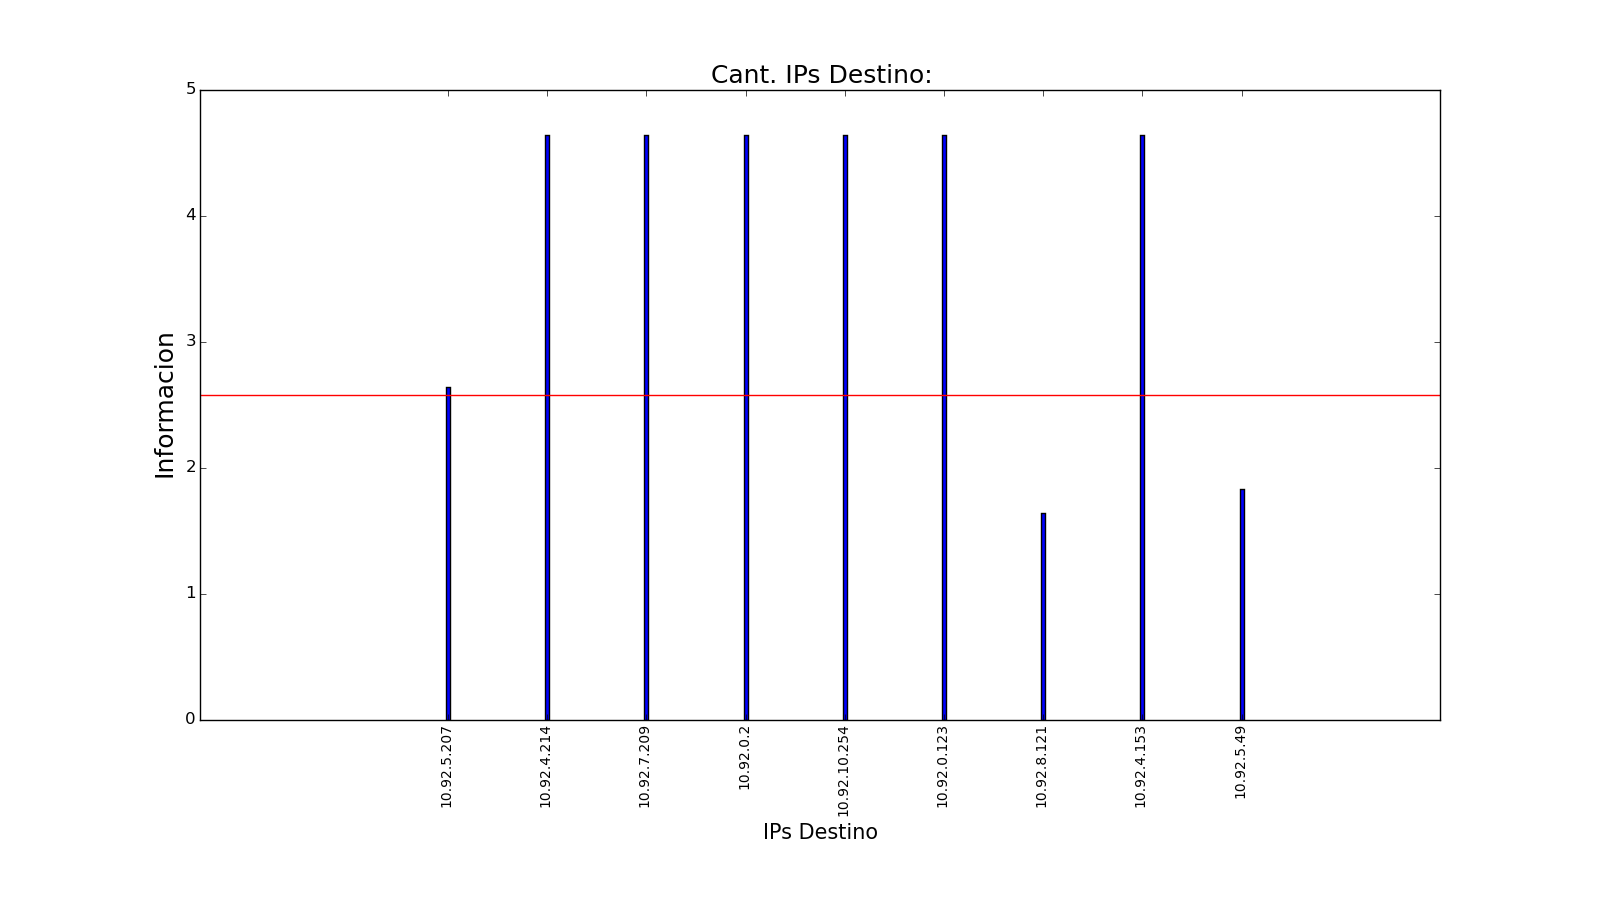
\includegraphics[width=1\textwidth]{../resultados/subte/histogram_dst_information.png}
       \caption{Información de IPs destino de los paquetes ARP}
       \label{red-Starbucks-dst-information}
\end{figure}

\begin{figure}[H]
       \centering
       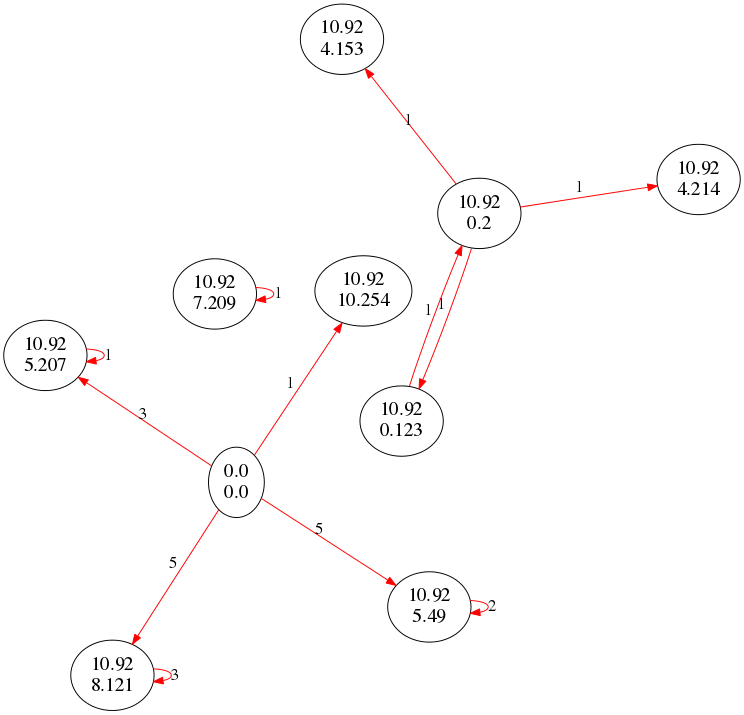
\includegraphics[width=1\textwidth]{../resultados/subte/network.png}
       \caption{Tráfico de paquetes ARP}
       \label{red-Starbucks-dst-information}
\end{figure}

Analizando los gráficos podemos ver que las IPs \textbf{10.92.8.121} y \textbf{10.92.5.49} reciben una mayor cantidad de paquetes que las demás y son nodos distinguidos por ser su información menor a la entropía. Pero los paquetes que reciben tienen como origen a la IP \textbf{0.0.0.0}, que como discutimos en la siguiente sección, son ARP requests que se mandan debido a la ejecución de un protocolo DHCP. No podemos sacar más conclusiones de estos gráficos debido al corto tiempo de intercepción de paquetes.\\
\newpage



\newpage
\section{Discusiones}


\newpage
\section{Conclusiones}

La primer conclusión a la que llegamos es que la teoría de la información se condice con la práctica; nos referimos a la relación entre la entropía de una fuente de información y los símbolos distinguidos (en nuestro caso IPs / Tipos de Paquete).

Resultó interesante analizar diversas redes, ya que pudimos ver comportamientos y complejidades distintas. Es más fácil analizar lo que pasa en una red hogareña, mientras que la transferencia de información en la red del laboratorio de Computación crece exponencialmente, y es más difícil analizar su estructura sin acceder a otra información.

Scapy nos resultó una herramienta fácil de implementar y utilizar, y cumplió su propósito.

Llegamos a la conclusión que no siempre los nodos distinguidos se corresponden con los routers de una red, aunque en nuestros casos casi siempre fue así. Sin embargo, habría sido interesante analizar una red ad hoc para evaluar su comportamiento.

Finalmente, pudimos observar que en ninguna de las redes analizadas se observa un overhead de paquetes ARP significativo, por ser la proporción de paquetes ARP pequeña respecto a la proporción del resto de los paquetes.




\end{document}
